\pdfminorversion=7
\documentclass[final]{beamer}
\mode<presentation> { }
\usepackage[english]{babel}
\usepackage[latin1]{inputenc}
\usepackage{amsmath,amsthm, amssymb, latexsym}
\usepackage{xspace}
\usepackage{tikz}
\usepackage{marvosym}
\usetikzlibrary{calc,shapes,arrows,shadows,fadings,positioning,backgrounds}
\usetikzlibrary{decorations.pathmorphing}
\usetikzlibrary{decorations.markings}
\usefonttheme[onlymath]{serif}
\boldmath
\usepackage[force]{feynmp-auto}


%Poster package
\usepackage[orientation=portrait,size=a0,scale=1.4,debug]{beamerposter}

%PDF information
\title{Exploring the high-energy frontier with the CMS detector}
\date{March 29th, 2019}


%Generators
\newcommand{\met}{\ensuremath{{\not\mathrel{E}}_T}}
\newcommand{\Madgraph}{M\scalebox{0.8}{AD}G\scalebox{0.8}{RAPH}\xspace} 
\newcommand{\Pythia}{P\scalebox{0.8}{YTHIA}\xspace} 
\newcommand{\Sherpa}{S\scalebox{0.8}{HERPA}\xspace} 
\newcommand{\Powheg}{P\scalebox{0.8}{OWHEG}\xspace} 
\newcommand{\Apacic}{A\scalebox{0.8}{PACIC++}\xspace} 
\newcommand{\MCFM}{\scalebox{0.8}{MCFM}\xspace} 

%Boundig box (set invisible)
\def\boxColor{red}
\def\oc{0}

%Remove margins
\setbeamersize{text margin left=0mm} 
\setbeamersize{text margin right=0mm} 
\renewcommand*{\arraystretch}{1.2}

%Graphics saved in...
\graphicspath{{figuren/}}
\setbeamertemplate{itemize items}{\color{black}$\bullet$}

\begin{document}

%Tikz styles
%\tikzstyle{boxStyle} = [very thick, fill=blue, rectangle, rounded corners=1cm, inner sep=10pt, inner ysep=20pt, opacity=0.05, text opacity=1, text width=\boxWidth]
%\tikzstyle{fancytitle} =[fill=blue!05, rounded corners, anchor=east,thick,draw]
\tikzstyle{boxStyle} = [very thick, fill=white, text=white, rectangle, rounded corners=1cm, inner sep=10pt, inner ysep=20pt, opacity=0.05, text opacity=1, text width=\boxWidth]
\tikzstyle{fancytitle} =[text=white, rounded corners, anchor=east,thick,draw, white]
\def\titleOffset{3cm}
\tikzstyle{insideBoxStyle} = [cyan, fill=white, text=black, ultra thick, rectangle, draw, rounded corners=2cm, inner sep=10pt, inner ysep=20pt, text width=\insideBoxWidth, font=\scriptsize]
\tikzstyle{insideFancytitle} =[text=white, rounded corners, font=\bfseries]
\def\insideTitleOffset{2cm}
\tikzfading[name=fade out,right color=transparent!100, middle color=transparent!100]

\tikzset{
    ultra thick/.style={line width=2mm}
}

%Avoid to much splitting of words in small boxes
\hyphenpenalty=1000

\frame{
  \vspace{-1cm}
  \makebox[\textwidth][c]{\begin{tikzpicture}[show background rectangle, background rectangle/.style={fill=black}]
    \node[opacity=0.15] (background) at (0,0){\includegraphics[width=150cm]{{background}.jpg}};
    \node[anchor=south] (LHC) at ($(background.north)-(0,5)$){\includegraphics[width=90cm, trim=0 150 0 100,clip]{{LHC}.jpg}};


    %title
    %\node[anchor=north west] (logoGhent) at (-43, 55) {\includegraphics[height=9cm]{{ugent}.eps}};
  %  \node[anchor=north east] (logoCMS) at (-30,-40) {\includegraphics[height=5cm]{{/usr/share/texmf/tex/latex/beamer/base/themes/theme/images/CMS-Color}.pdf}};
    \node[anchor=north,font=\Large, text width=80cm,align=center] (title) at (LHC.south){\color{white}\fontsize{110}{140}\textbf{CMS: Expedition into the high-energy frontier}};
    \node[anchor=south east,font=\Large, text width=80cm,align=right] (title) at ($(LHC.south east)+(-7,1)$){\color{black}\textbf{Prof. D. Dobur}\\ ddidar@cern.ch};

    
        \def\cmsBoxWidth{43cm}
    \def\firstRowHeight{31cm}
    \node[boxStyle, text width=\cmsBoxWidth, anchor=north west, minimum height=\firstRowHeight] (cmsBox) at (-40, 41){
       \begin{minipage}{\cmsBoxWidth}
          {\small
          The \textbf{Compact Muon Solenoid (CMS) experiment} is a particle-physics experiment at the \textbf{Large Hadron Collider} (LHC), the world's most powerful particle accelerator located at CERN, Geneva.
          CMS is designed to detect a wide range of particles and phenomena produced in the LHC's high-energy proton-proton collisions. During its first years of operation, CMS achieved many new precision results on
          the Standard Model and limits on new physics beyond the Standard Model, as well as the long awaited discovery of the Higgs boson.
          In the previous years (2015-2018), CMS took data at an \textbf{unprecedented centre-of-mass energy of 13 TeV}, and at a rate of 40 million collisions per second.
          In your master thesis, you will use these data for precision measurements or searches for new physics, acquiring useful knowledge of data analysis
          techniques for your future academic or professional career!
          \vspace{5mm}
          \begin{figure}
            \centering
             \includegraphics[height=12cm,trim=50 0 50 0,clip]{{CMS}.jpg}      
             \hspace{2cm}
             \includegraphics[height=12cm]{{ed2}.png}   
          \end{figure}
          \vspace{5mm}
          \color{white} The CMS experiment is one of the largest international scientific collaborations in history, involving 4300 particle physicists, engineers, technicians, students and support staff from 229 universities and institutes in 51 countries.
       }\end{minipage}
   };
   \node[green] at ($(cmsBox.south east)+(-14,18.3)$){$e$};
   \node[green] at ($(cmsBox.south east)+(-7.2,11.7)$){$e$};
   \node[red] at ($(cmsBox.south east)+(-4,8)$){$\mu$};
   \node[red] at ($(cmsBox.south east)+(-4,18)$){$\mu$};


 %   \node[fancytitle, left=\titleOffset] at (cmsBox.north east) {The CMS detector at the LHC};


   %     \def\subjectBoxWidth{80cm}
    \def\cmsBoxWidth{110cm}
    \def\middleRowHeight{11cm}
    \node[boxStyle, draw, color=cyan, opacity=1, fill opacity=0.05, ultra thick, fill=white, text width=\subjectBoxWidth, anchor=north west, minimum height=\middleRowHeight] (photonBox) at  ($(cmsBox.south west)+(0,-1.5)$){
        \centering
        \hspace{2cm}
        \begin{minipage}{20cm}
        \includegraphics[height=10.5cm]{{gg}.png}
        \end{minipage}
        \hspace{2cm}
        \begin{minipage}{12cm}
                \includegraphics[height=10.5cm]{{ggATLAS}.png}
        \end{minipage}
        \begin{minipage}{37cm}
         \small
         \color{white}
         The analysis of the 2015 data shows an interesting \textquotedblleft bump \textquotedblright in the $M(\gamma\gamma$) spectrum that hints to a new particle with a mass of $\sim$750 GeV.
         If  the upcoming data confirms this hint, a new era in the history of particle physics might begin.
         You can take part in this exciting journey with your master thesis and witness the dawn of a new age.
        \end{minipage}
        };
 %   \node[fancytitle, left=\titleOffset] at (cmsBox.north east) {The CMS detector at the LHC};
     \node[green] at ($(photonBox.north west)+(14.5,-1)$){$\gamma$};
     \node[green] at ($(photonBox.north west)+(17.5,-8)$){$\gamma$};



    \node[opacity=0.12,anchor=east] (background) at ($(cmsBox.south east)-(3,2)$){\includegraphics[width=20cm]{{DeathStar2}.jpg}};
    {
    \def\subBoxWidth{38cm}
    \def\subjectBoxWidth{80cm}
    \def\subjectRowHeight{53.5cm}
    \def\topRowHeightLeft{16.5cm}
    \def\topRowHeightRight{22.5cm}
    \def\bottomRowHeightLeft{23.5cm}
    \def\bottomRowHeightRight{17.5cm}
    \node[anchor=north west, boxStyle, text width=\subjectBoxWidth, anchor=north west, minimum height=\subjectRowHeight] (subjects) at ($(cmsBox.south west)+(0,-1.5)$){
    };

    \node[anchor=north,color=white, text width=70cm] at ($(subjects.north)+(0,-.5)$){
          \small
          The Ghent CMS team is involved in several analyses at CMS, which include supersymmetry searches, top quark physics, and searches for heavy neutral leptons.
          Master students are welcome to join in one of our analyses groups where they get the opportunity to explore the large amounts of new data.
          Under the daily supervision of our CMS team, you will acquire the necessary knowledge to identify particles, select the events of interest and to use big data analysis techniques.
          You get the opportunity to gain experience in an international collaboration, and present/discuss results at CERN.
    };
    
    
    
    

    
    
    
    \node[insideBoxStyle, text width=\subBoxWidth, anchor=north east,minimum height=\topRowHeightLeft] (box1) at ($(subjects.north)+(-1,-10)$){
       \hspace{0.5cm}
       \begin{minipage}{35cm}
         \textbf{Search for the flavour-changing neutral Higgs interactions with top quarks at CMS}\\
         Flavour-changing neutral currents (FCNC) are among the rarest processes in the Standard Model (SM). 
         The probe of the FCNC interactions of a top quark with a Higgs boson represents an excellent probe of various beyond the SM theories. 
         The study includes the search for the top quark FCNC decays in the top quark pair production process, 
         as well as the probe of FCNC effects in the single top associated production with a Higgs boson. 
         One of the tasks in this analysis is to develop an event selection criteria to identify the FCNC processes 
         with a potential use of various Machine Learning techniques. 
       \end{minipage}\\
       \hspace{2.5cm}
       \begin{minipage}{15cm}
         \begin{center}
         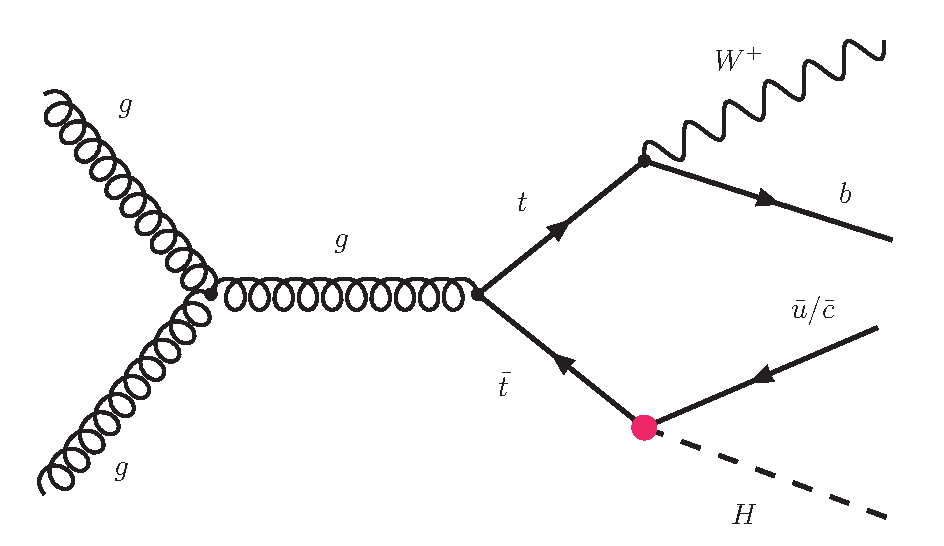
\includegraphics[width=0.9\textwidth]{fcnc/tH_ttbar_mod.eps} 
         \end{center}
       \end{minipage}
       \hspace{2cm}
       \begin{minipage}{15cm}
         \begin{center}
         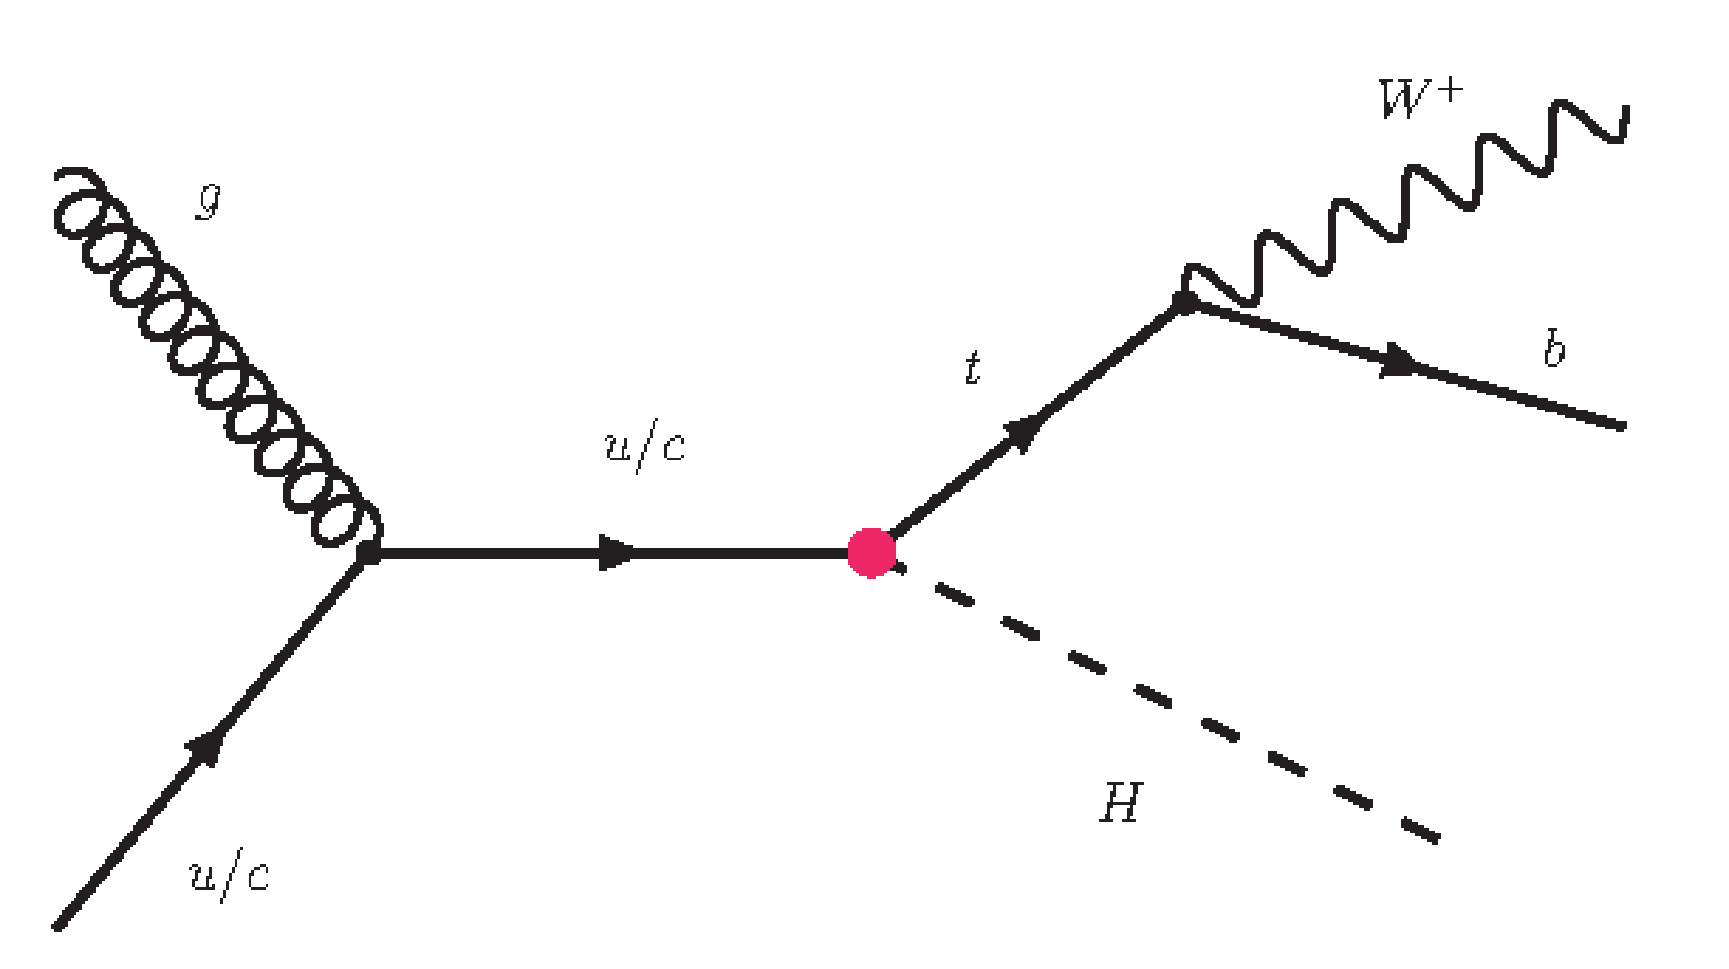
\includegraphics[width=0.9\textwidth]{fcnc/tH_mod.eps} 
         \end{center}
       \end{minipage}
    };
    \node[insideFancytitle, left=\insideTitleOffset] at ($(box1.north east)+(0,0.5)$){\normalsize Flavour changing neutral currents}; 
   
 

    \node[insideBoxStyle, text width=\subBoxWidth, anchor=north west,minimum height=\bottomRowHeightLeft] (box2) at ($(box1.south west)+(0,-2.5)$){
        \hspace{0.5cm}
        \begin{minipage}{22cm}
          \textbf{A study of displaced tracking efficiency using neutral kaon decays in the CMS detector}\\
          The CMS detector at the CERN LHC was designed for the detection and accurate reconstruction of particles 
          emerging directly from the proton-proton collisions at the detector center. 
          However, some extensions to the standard model of particle physics include undetectable particles that only 
          decay to detectable particles at a relatively large distance from the detector center. 
          The goal of this thesis project is to quantify the efficiency of the CMS detector for this kind of so-called displaced objects, 
          using a partly data-driven technique. The focus will be on the decay of the neutral K-meson to two charged pions. 
          Since the K-meson itself is invisible to the inner part of the detector and has a relatively long lifetime, 
          its decay to two pions yields a similar signature as the exotic `beyond standard model` scenarios one is typically investigating. 
          Using both simulated events and actual data, we will try to measure the efficiency of CMS for measuring displaced decays and 
          estimate the uncertainty on this measurement. 
        \end{minipage}
        \begin{minipage}{13cm}
        \begin{center}
          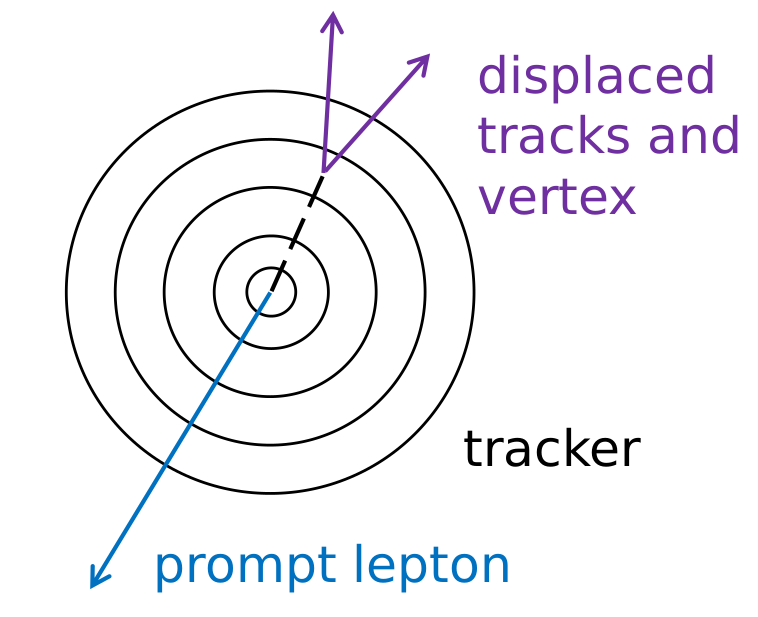
\includegraphics[width=0.9\textwidth]{displacedTracking/displacedTracks.png} \\
          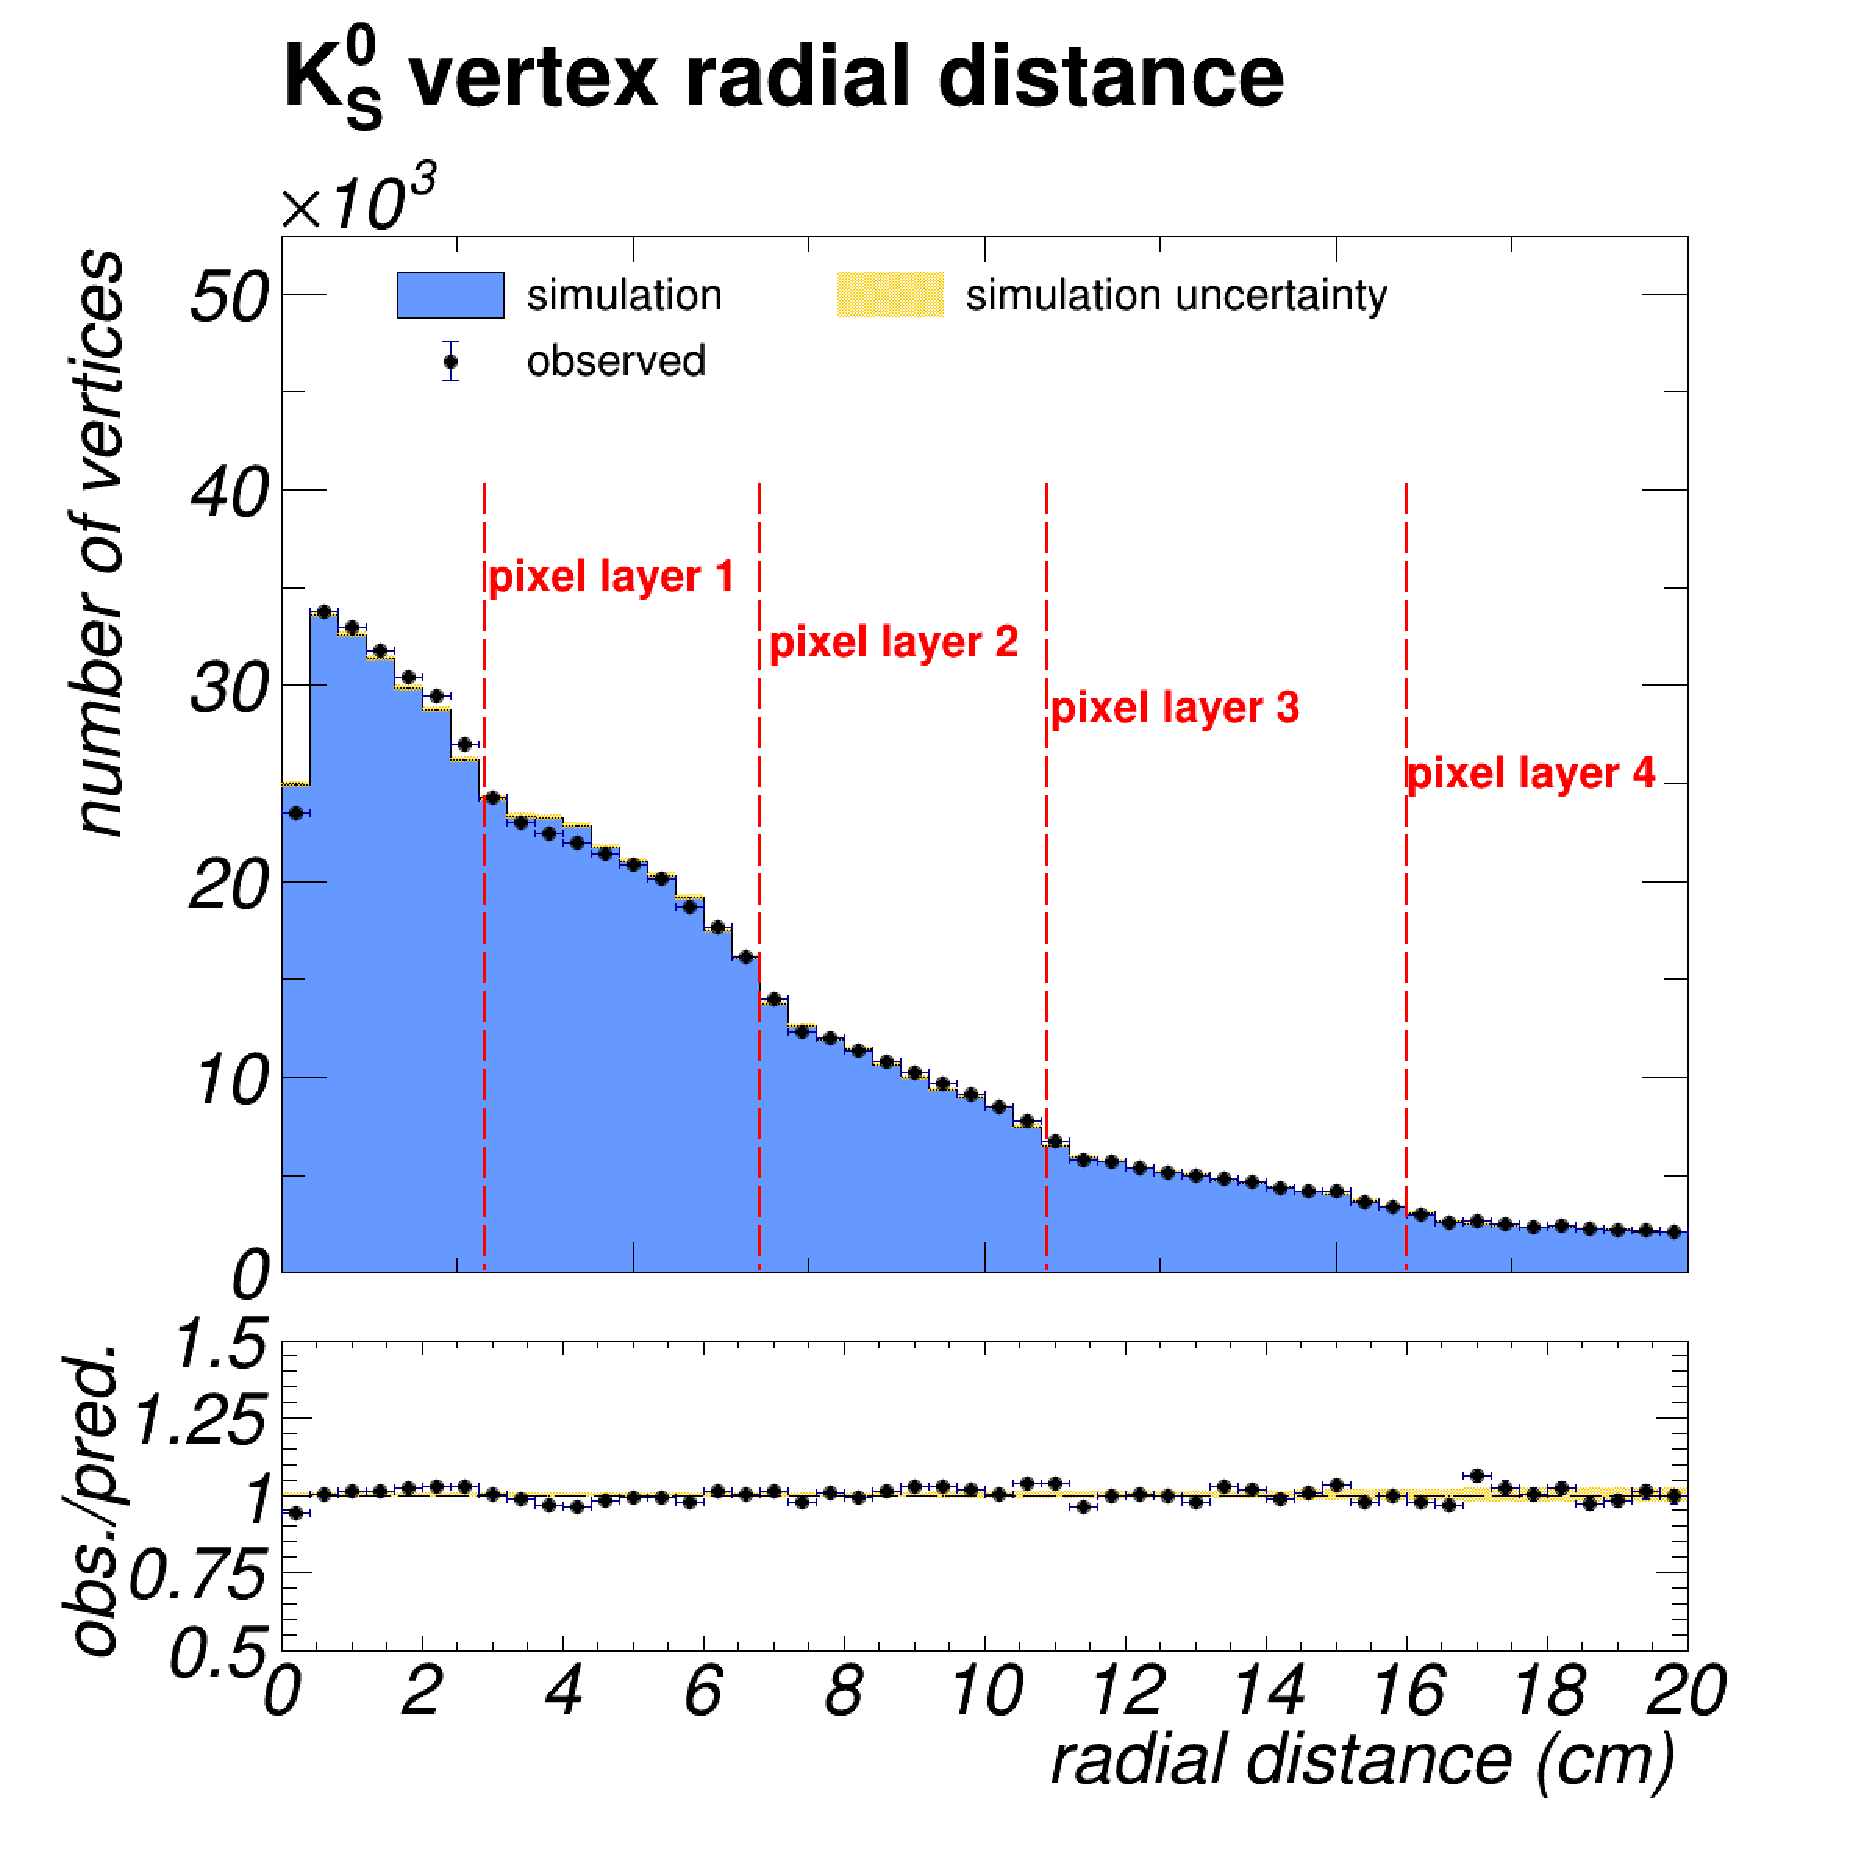
\includegraphics[width=0.9\textwidth]{displacedTracking/2017E_detector.pdf} 
        \end{center}
        \end{minipage}

    };
    \node[insideFancytitle, left=\insideTitleOffset] at ($(box2.north east)+(0,0.5)$){\normalsize Tracking};
     
 
 

   
   
    \node[insideBoxStyle, text width=\subBoxWidth, anchor=north west,minimum height=\topRowHeightRight] (box3) at ($(subjects.north)+(1,-10)$){
       \hspace{0.5cm}
       \begin{minipage}{35cm}
         \textbf{Rediscovering the Higgs boson at CMS}\\
         The exact mass generation mechanism still remains to be an open question in particle physics. 
         The study of the Higgs boson production represents the direct probe of the Higgs boson couplings to other fundamental constituents of nature. 
         Any deviations in the measured values of these parameters from the SM predictions would directly point to the new physics phenomena. 
         The study is proposed for the analysis of the CMS detector data to rediscover the Higgs boson in one of its production processes
         by additionally involving Machine Learning techniques to further boost the final sensitivity in the analysis. 
       \end{minipage}
       \begin{center}
         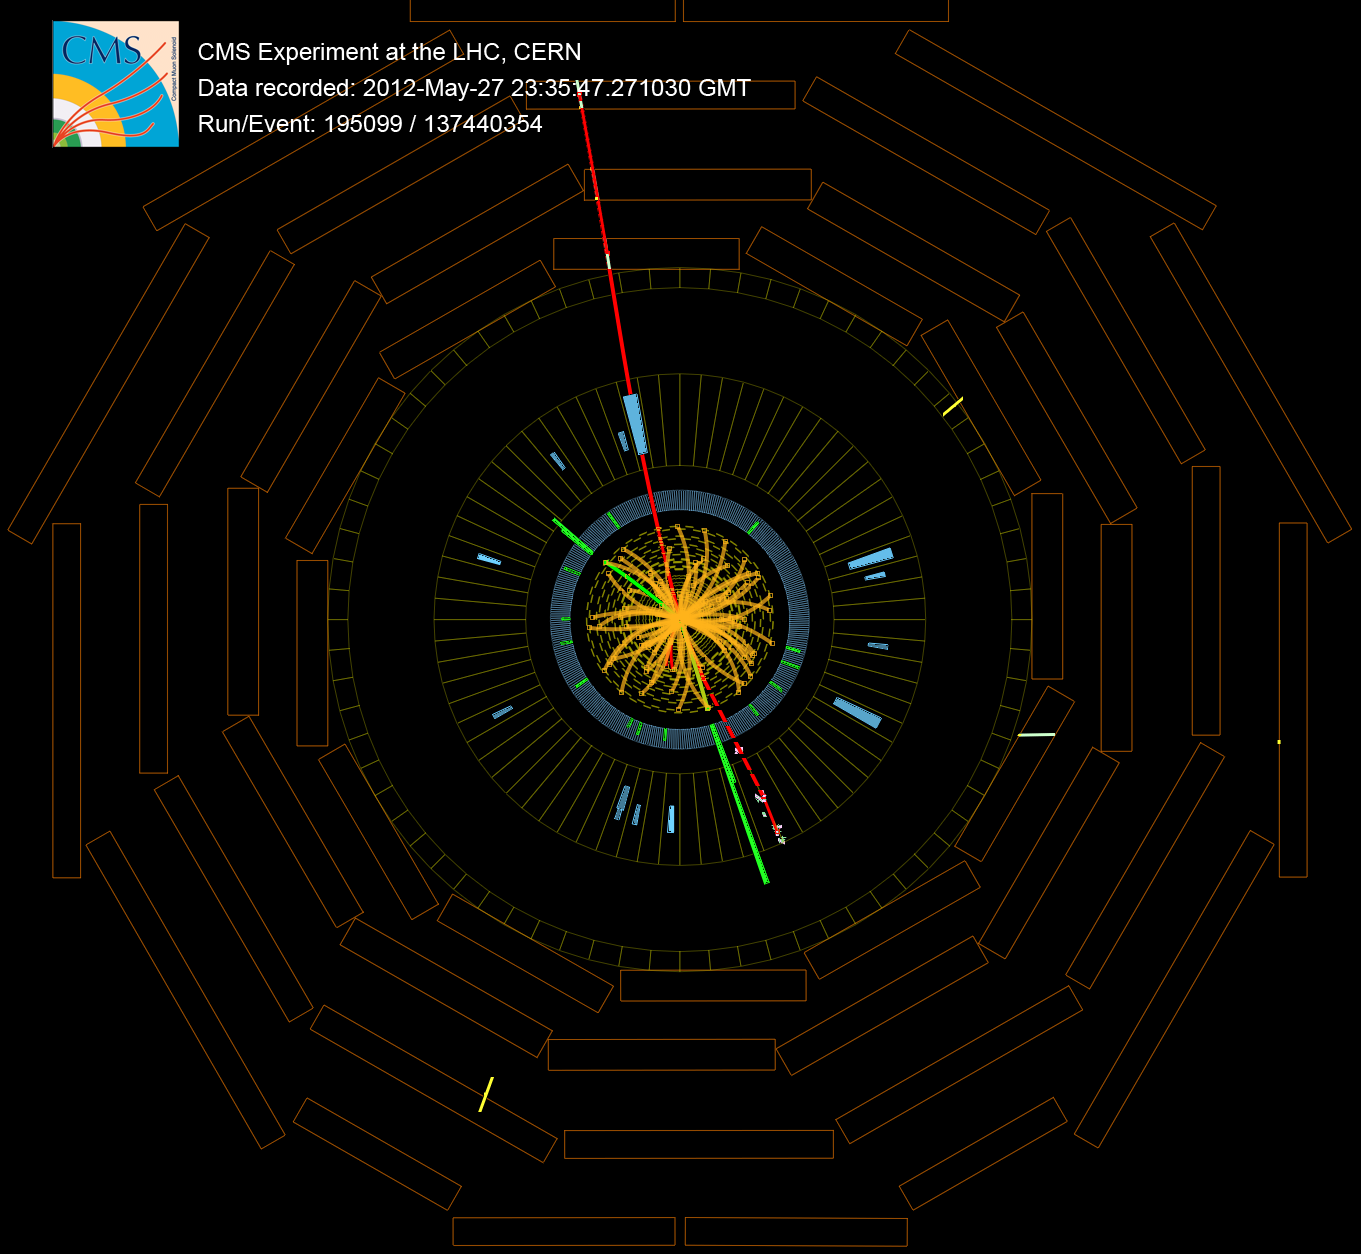
\includegraphics[height=13cm]{higgs/higgs.png} 
         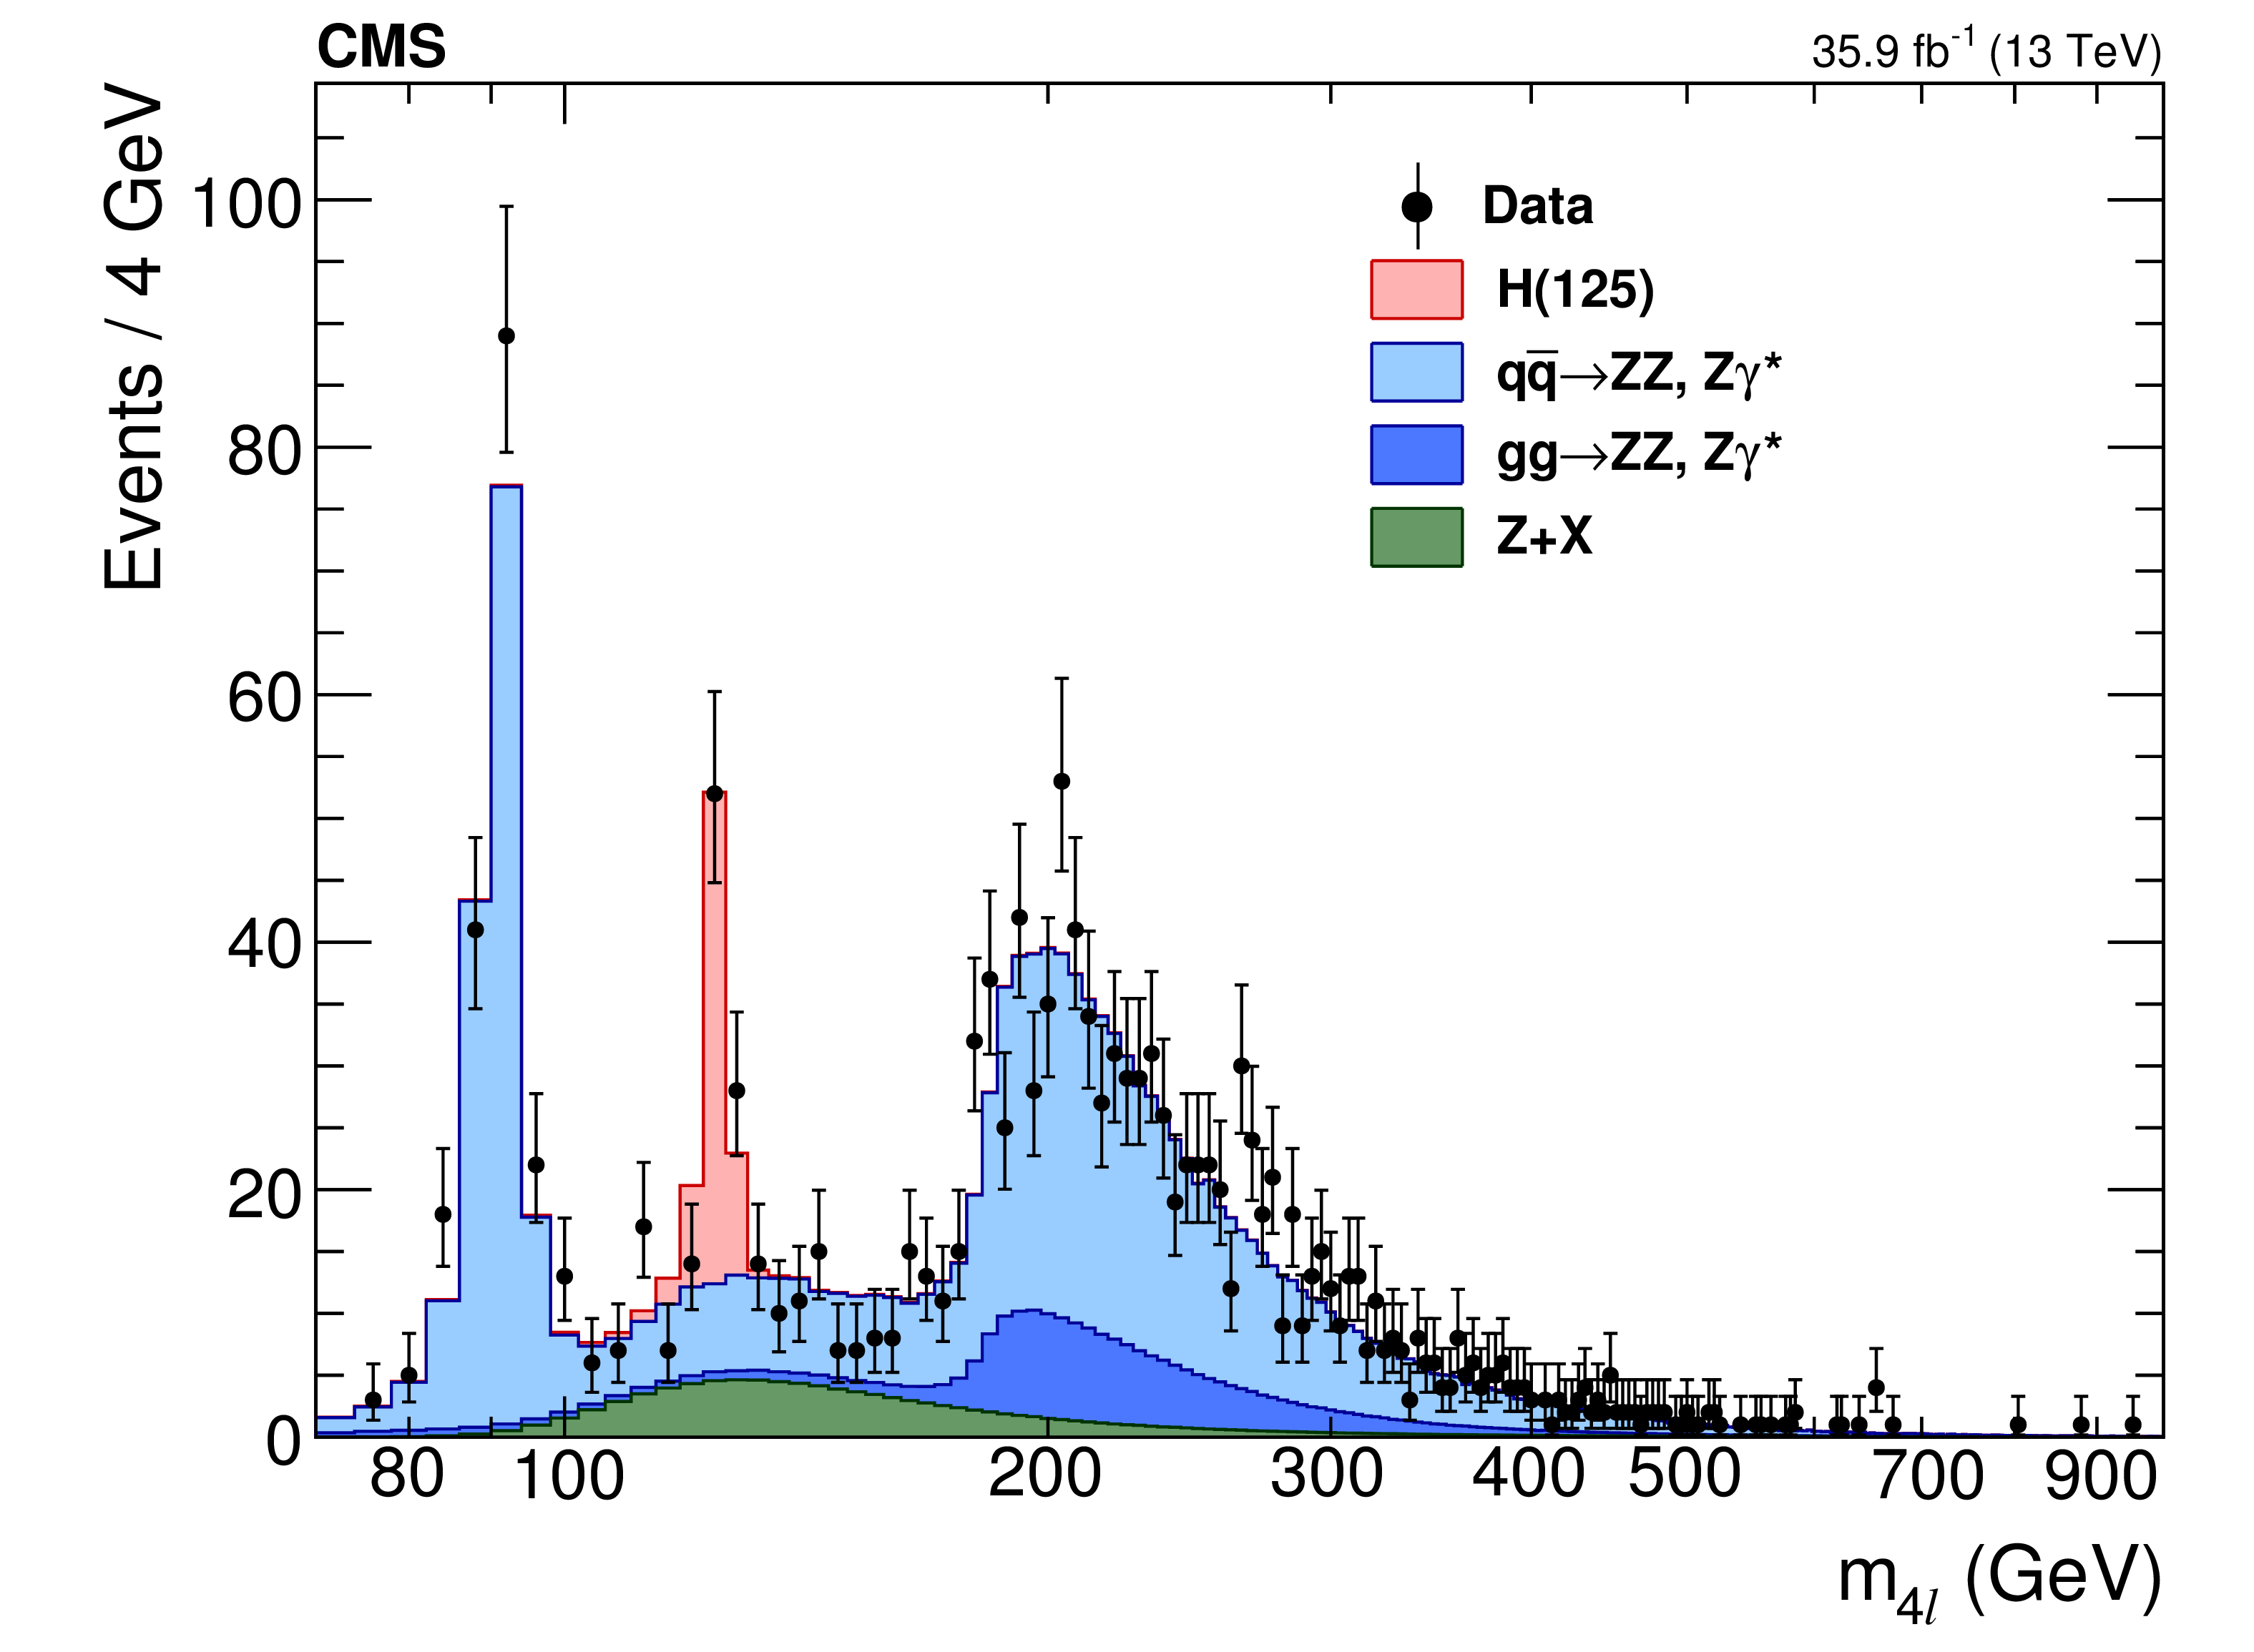
\includegraphics[height=13cm]{higgs/higgs2.png} 
       \end{center}
    };
    \node[insideFancytitle, left=\insideTitleOffset] at ($(box3.north east)+(0,0.5)$){\normalsize Rediscovering the Higgs boson at CMS};
    

    \node[insideBoxStyle, text width=\subBoxWidth, anchor=north east,minimum height=\bottomRowHeightRight] (box4) at ($(box3.south east)+(0,-2.5)$){
       \hspace{0.5cm}
       \begin{minipage}{25cm}
         \textbf{Enlightening the top quark: a study of the interaction of a top quark and a photon with the CMS detector}\\
         The distinctive properties of the top quark put it in a special place of the Standard Model (SM).
         A precise study of the strength of the interaction of this particle with other fundamental constituents 
         represents an important test of the SM predictions. The study of the processes with the production 
         of a top quark in association with a photon represents a direct probe of the electroweak charge and interaction couplings of the top quark, 
         as well as provides a handle to search for various new physics effects. 
         The proposed analysis will cover the study of the kinematic properties of the processes with the production of top quark pairs 
         with one or more photons in the final state with the CMS detector. 
         The possible tasks include the study of the photon identification in data, 
         as well as the development of the event selection criteria exploiting the full event reconstruction. 
         A potential gain from the use of Machine Learning techniques will also be explored. 
       \end{minipage}
       \begin{minipage}{9cm}
       \begin{center}
         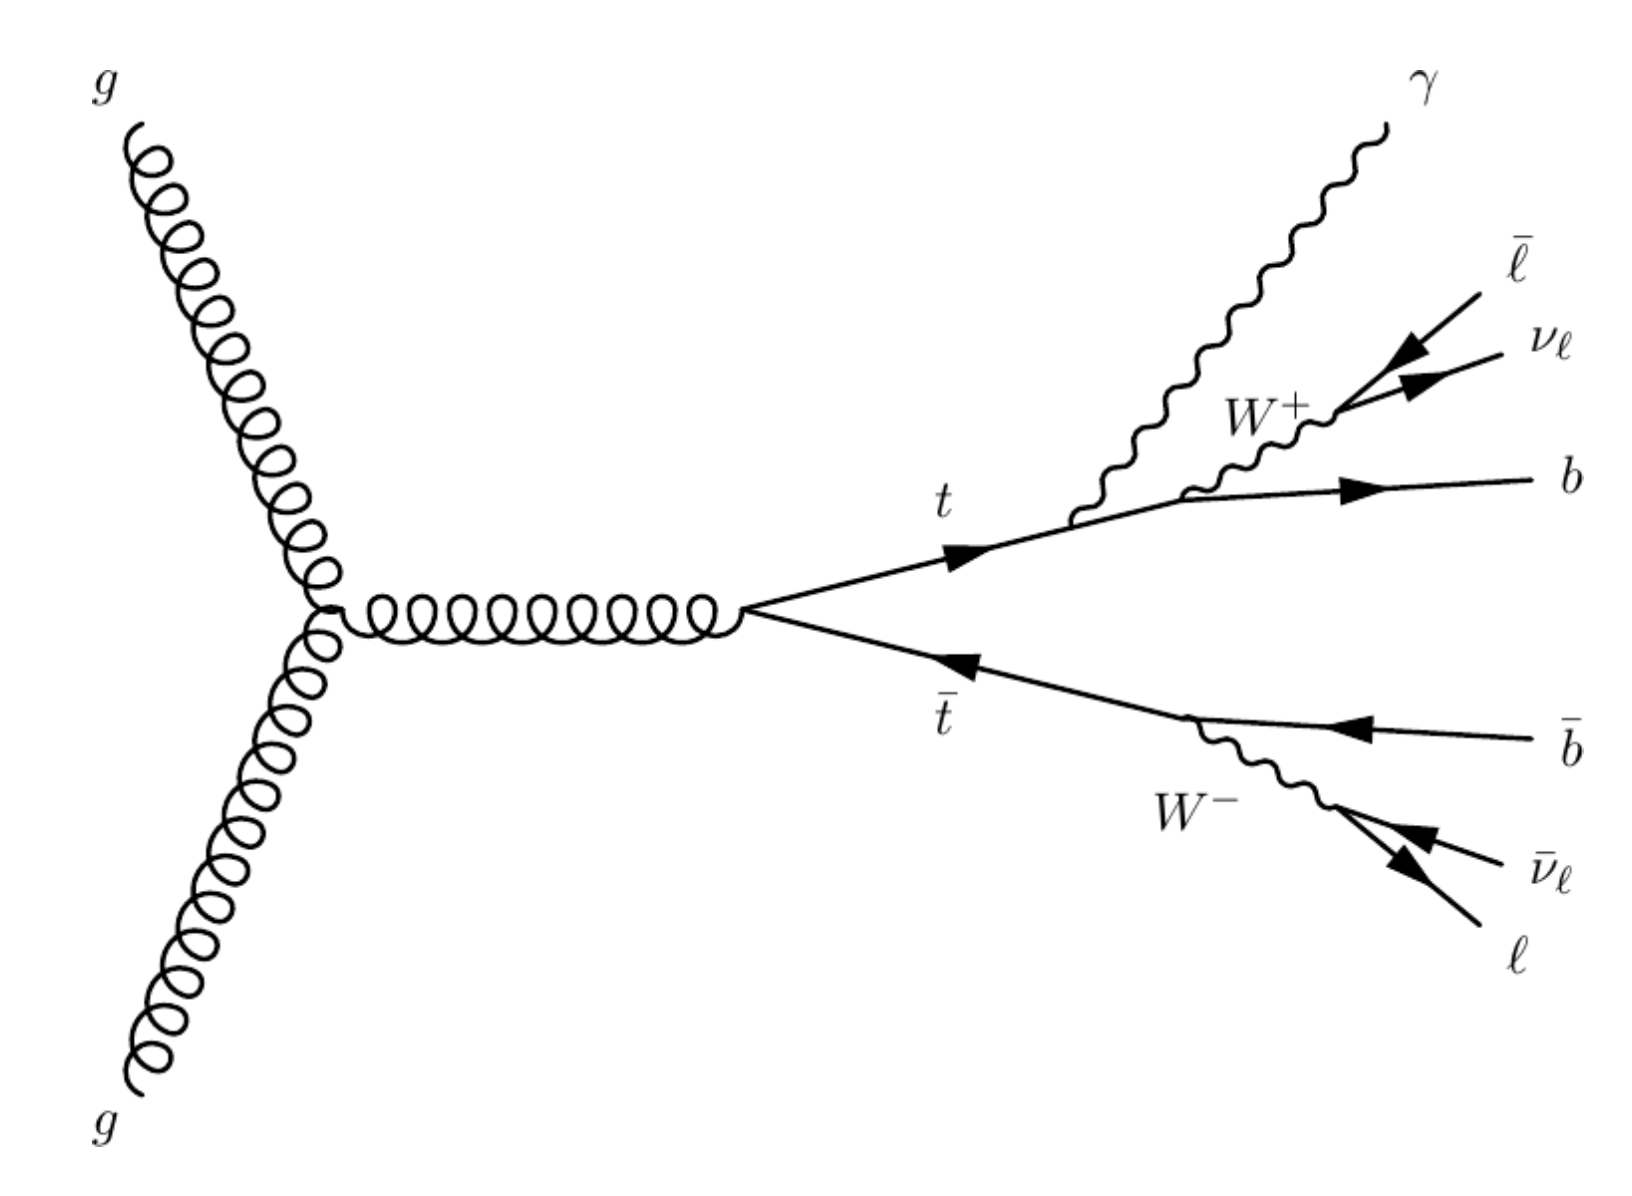
\includegraphics[width=0.9\textwidth]{ttgamma/diagram.png} 
       \end{center}
       \end{minipage}
    };
    \node[insideFancytitle, left=\insideTitleOffset] at ($(box4.north east)+(0,0.5)$){\normalsize Interaction of a top quark and a photon}; 
    
    
       
       

}
        \def\ugentBoxWidth{33cm}
    \node[boxStyle, text width=\ugentBoxWidth, anchor=north east, minimum height=\firstRowHeight] (ugentBox) at (cmsBox.north -| subjects.east){
       \begin{minipage}{33cm}
        \begin{figure}
           \includegraphics[width=15cm,trim=25 25 25 25,clip]{{particles}.png}         
           \includegraphics[width=15cm,trim=25 25 25 25,clip]{{pf}.png}           
          \end{figure}
          \color{white}
          \small
         Multiple observations and the everyday experience of gravity hint at the fact that the Standard Model (SM) is not the ultimate theory of nature. Why is the Higgs boson so light? Why is matter so abundant compared to antimatter? Why is gravity so much weaker than the other forces? How can neutrinos be so light?
New data, never before explored, might hold keys to unlocking these secrets about the fundamental nature of nature itself! Data collected in the recently finished Run II, at the never aforetime reached energy of 13 TeV, will provide a matchless opportunity for joining this expedition into the high energy frontier. There are several available thesis subjects focussed on analysing the many uncharted dwellings in the LHC's data, all complementary to the research being performed in the Gent CMS group.
       \end{minipage}

    };
 %   \node[fancytitle, left=\titleOffset] at (ugentBox.north east) {Data analysis at CMS};



    
    \node[text width=50cm, align=center,font=\scriptsize] at (0,-46.5){\color{white}\textbf{Ghent CMS Group, Campus Proeftuin, N3, https://epp.ugent.be/index.php/masterthesesubjects/}};

    
  \end{tikzpicture}}
}
\end{document}